\chapter{Embedded implementation}
\label{ch:Embedded}
In \autoref{ch:Framework}, an overview of the framework developed in \texttt{python} was given, relying on the \gls{glo:mongodb} database. This chapter will focus on the implementation of the embedded system. The first big difference is that the embedded system is written in \texttt{C}, that is not an object oriented language. The second big difference is that the embedded system is not using a database, but it relies only on the variables stored in the RAM. Because of the memory constraints, the training phase relies with the comunication with a pc for storing the heavy data. Once the model has been trained, the model is stored in the embedded program and the novelty detection is performed in real time. The general structure is shown in \autoref{fig:Embedded}.

\begin{figure}
    \centering
    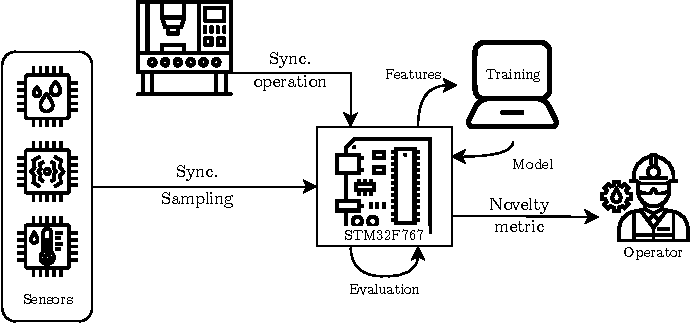
\includegraphics[scale=1]{images/Embedded/EmbeddedStructure.pdf}
    \caption{Embedded system overview}
    \label{fig:Embedded}
\end{figure}